%% Green-X — Science of the Total Environment manuscript (Elsevier elsarticle).
%% STOTEN conventions: author-year (Harvard) citations, double-spaced
%% line-numbered review layout, abstract <= 300 words, 5 highlights (<= 85
%% chars each), <= 6 keywords, graphical abstract at submission.
%% Build: latexmk -pdf main.tex
%% Sections live in contents/0N_*.tex; figures come from ../../Model/paper_figures/.
\documentclass[review,12pt,authoryear]{elsarticle}

\usepackage{graphicx}
\usepackage{booktabs}
\usepackage{amsmath}
\usepackage{lineno}
\usepackage[hidelinks]{hyperref}
\graphicspath{{figures/}}
\linenumbers

\journal{Science of the Total Environment}

\begin{document}

\begin{frontmatter}

\title{Interpolation versus generalization in machine learning prediction
of micropollutant adsorption on layered double hydroxides}

%% Authors intentionally left for the user to fill in.
\author[inst1]{[AUTHORS TO BE ADDED]}
\affiliation[inst1]{organization={[AFFILIATION]}, country={[COUNTRY]}}

\begin{abstract}
%% One paragraph, 300--340 words, quantified. All values trace to
%% Model/paper_figures/*.csv and Model/interp_row_42/ (see CLAIMS.md).
Micropollutants such as pharmaceuticals, pesticides, and personal-care
products are detected in water bodies worldwide, and layered double
hydroxides (LDHs) are widely studied as tunable adsorbents for their
removal.
Machine learning (ML) models trained on literature-compiled datasets
increasingly report near-perfect prediction of adsorption performance, yet
the evaluation protocols behind these reports rarely account for the
structure of the underlying data, in which many experimental records
originate from few source studies. We compiled 1,342 adsorption experiments
for LDH--micropollutant systems from 59 published studies and evaluated
seven regression models (linear regression, $k$-nearest neighbors, neural
network, Cubist, random forest, XGBoost, and histogram gradient boosting)
under a leakage-aware protocol that separates two questions: interpolation
within studied systems and generalization to unseen studies. With
duplicate records removed and all preprocessing fitted on training folds
only, the best model predicted removal ratio (RR\%) for studied systems at
new operating conditions with $R^2$ of 0.87 and RMSE of 10 percentage
points. Under leave-one-study-out evaluation, however, the median
per-study error rose to 14--16 percentage points, two to three times the
interpolation error, and only 20 of the 59 studies were predicted with
accuracy resembling the interpolation regime, showing that random-split
protocols overstate the screening ability of literature-trained models by
a wide margin; the models still reduce the error of descriptor-free
baselines by roughly 40 percent, so some signal does transfer. Split-conformal prediction intervals certified the
interpolation task (93\% empirical coverage at a 90\% nominal level, with
$\pm$19-point intervals), but for unseen studies the intervals had to
widen to $\pm$68 points to maintain coverage, and a common
distance-to-training applicability score carried no information about
realized error in either task. Chemistry-informed features, including
the electrostatic driving force pH$-$pH$_{\mathrm{pzc}}$, changed the
errors little yet yielded feature attributions consistent with
electrostatic and hydrophobic adsorption mechanisms. The results
delimit what literature-trained adsorption models can currently support
in practice: condition optimization for studied systems, but not yet the
screening of new adsorbent--pollutant combinations.
\end{abstract}

%%\begin{graphicalabstract}
%%\includegraphics{grabs}  % placeholder -- to be produced at submission
%%\end{graphicalabstract}

\begin{highlights}
\item 1,342 LDH adsorption records from 59 studies evaluated leakage-aware
\item Random splits overstate ML skill: $R^2$ 0.85 within studies, near zero across
\item Leave-one-study-out audit quantifies transfer for every source study
\item Conformal intervals certify interpolation; new-study intervals widen 3--4$\times$
\item pH$-$pH$_{\mathrm{pzc}}$ feature links model behavior to electrostatics
\end{highlights}

\begin{keyword}
layered double hydroxide \sep micropollutant \sep adsorption \sep machine
learning \sep data leakage \sep uncertainty quantification
\end{keyword}

\end{frontmatter}

\section*{Nomenclature}
\begin{tabular}{@{}ll@{}}
LDH & layered double hydroxide \\
RR\% & removal ratio (percent) \\
$C_i$ & initial concentration (mg/L) \\
AD & adsorbent dose (g/L) \\
pH$_{\mathrm{pzc}}$ & pH at the point of zero charge \\
BET & Brunauer--Emmett--Teller surface area (m$^2$/g) \\
PV & pore volume (cm$^3$/g) \\
APD & average pore diameter (nm) \\
$d_{003}$ & basal interlayer spacing (nm) \\
log $K_{\mathrm{ow}}$ & octanol--water partition coefficient \\
ML & machine learning \\
LR, KNN, ANN & linear regression, $k$-nearest neighbors, neural network \\
RF, XGB, HistGB & random forest, XGBoost, histogram gradient boosting \\
LOSO & leave-one-study-out \\
(T1), (T2) & interpolation task, cross-study generalization task \\
MAE, RMSE & mean absolute error, root mean square error \\
SHAP & Shapley additive explanations \\
CV & cross-validation \\
\end{tabular}

\section{Introduction}
\label{sec:intro}

Micropollutants, including pharmaceuticals, pesticides, endocrine
disruptors, and personal-care products, are detected at ng/L to \textmu g/L
levels in surface water, groundwater, and treated effluent worldwide
\citep{TODO-micropollutant-occurrence}. Conventional treatment trains
remove many of these compounds only partially, and their chronic ecological
and human-health effects have placed micropollutant control on regulatory
agendas in the European Union, the United States, and Asia
\citep{TODO-regulation}. Adsorption is among the most widely deployed
polishing steps because it requires no reagent input, produces no
transformation by-products, and operates across wide concentration ranges
\citep{TODO-adsorption-review}.

Layered double hydroxides (LDHs) are a class of anionic clays with the
general formula
$[\mathrm{M}^{2+}_{1-x}\mathrm{M}^{3+}_{x}(\mathrm{OH})_2]^{x+}
[\mathrm{A}^{n-}]_{x/n}\cdot m\mathrm{H_2O}$, whose metal composition,
interlayer anion, and calcination state can be tuned to target specific
pollutants \citep{TODO-ldh-review}. Hundreds of LDH variants have been
synthesized and tested against individual micropollutants, and each such
study reports removal under its own grid of pH, temperature, contact time,
adsorbent dose, and initial concentration. The resulting literature is
large but fragmented: no single laboratory can cover the combinatorial
space of metal pairs, synthesis routes, and pollutants experimentally.

Isotherm and kinetic models describe each of these systems in isolation
and offer no mechanism for pooling evidence across studies. Machine
learning (ML) offers a natural response to this fragmentation.
By compiling published experiments into a single dataset, ML models have
been trained to predict adsorption capacity or removal ratio from
material, pollutant, and operating descriptors, with reported test
$R^2$ values frequently above 0.9
\citep{TODO-ml-adsorption-1, TODO-ml-adsorption-2, TODO-biochar-cubist}.
Such models promise two distinct services: interpolating the behavior of
an already-studied adsorbent--pollutant system at untested conditions, and
screening new systems before synthesis. The second service is the one
most frequently invoked to motivate these studies.

However, we argue that the evaluation protocols behind these reports do
not support the screening claim. Firstly, literature-compiled datasets
are strongly clustered: in our compilation, 1,342 experimental records
originate from only 59 source studies, and within one study the material
and pollutant descriptors are constant while only operating conditions
vary. A random record-level train--test split therefore places
near-duplicate records on both sides, and the test score measures
within-study interpolation while being reported as generalization.
Secondly, preprocessing steps such as imputation, scaling, and feature
selection are commonly fitted on the full dataset before splitting, which
leaks test-set information into training \citep{kapoor2023leakage}.
Thirdly, point predictions are reported without uncertainty estimates or
applicability bounds, leaving practitioners no way to know when a
prediction should be trusted.

To address the above challenges, we evaluate ML models for micropollutant
adsorption on LDHs under a protocol that closes each of these leakage
pathways. In essence, our idea is
to treat the source study as the unit of generalization: we evaluate every
model twice, once under a duplicate-free record-level split that answers
the interpolation question, and once under grouped, leave-one-study-out
protocols that answer the screening question, with all preprocessing
confined to training folds in both cases. We complement point predictions
with split-conformal intervals and a distance-based applicability-domain
score, and we examine whether chemistry-informed features improve
cross-study transfer.

More specifically, this study aims to (1) quantify the gap between
interpolation and cross-study generalization for seven regression models
on 1,342 LDH--micropollutant records from 59 studies; (2) equip the
predictions with distribution-free uncertainty intervals and an
applicability-domain flag, and test their reliability under both tasks;
and (3) evaluate chemistry-informed features, including the electrostatic
driving force pH$-$pH$_{\mathrm{pzc}}$, and read the resulting feature
attributions against known adsorption mechanisms. To the best of our
knowledge, this is the first study of LDH adsorption modeling that
separates these two prediction tasks explicitly and reports what
literature-trained models can, and cannot yet, deliver for practice.

\section{Materials and methods}
\label{sec:methods}

Figure~\ref{fig:workflow} summarizes the workflow: compilation and
cleaning of the literature data, the two-task evaluation protocol,
leakage-controlled model pipelines, and the uncertainty and
interpretation layers.

\begin{figure}[t]
\centering
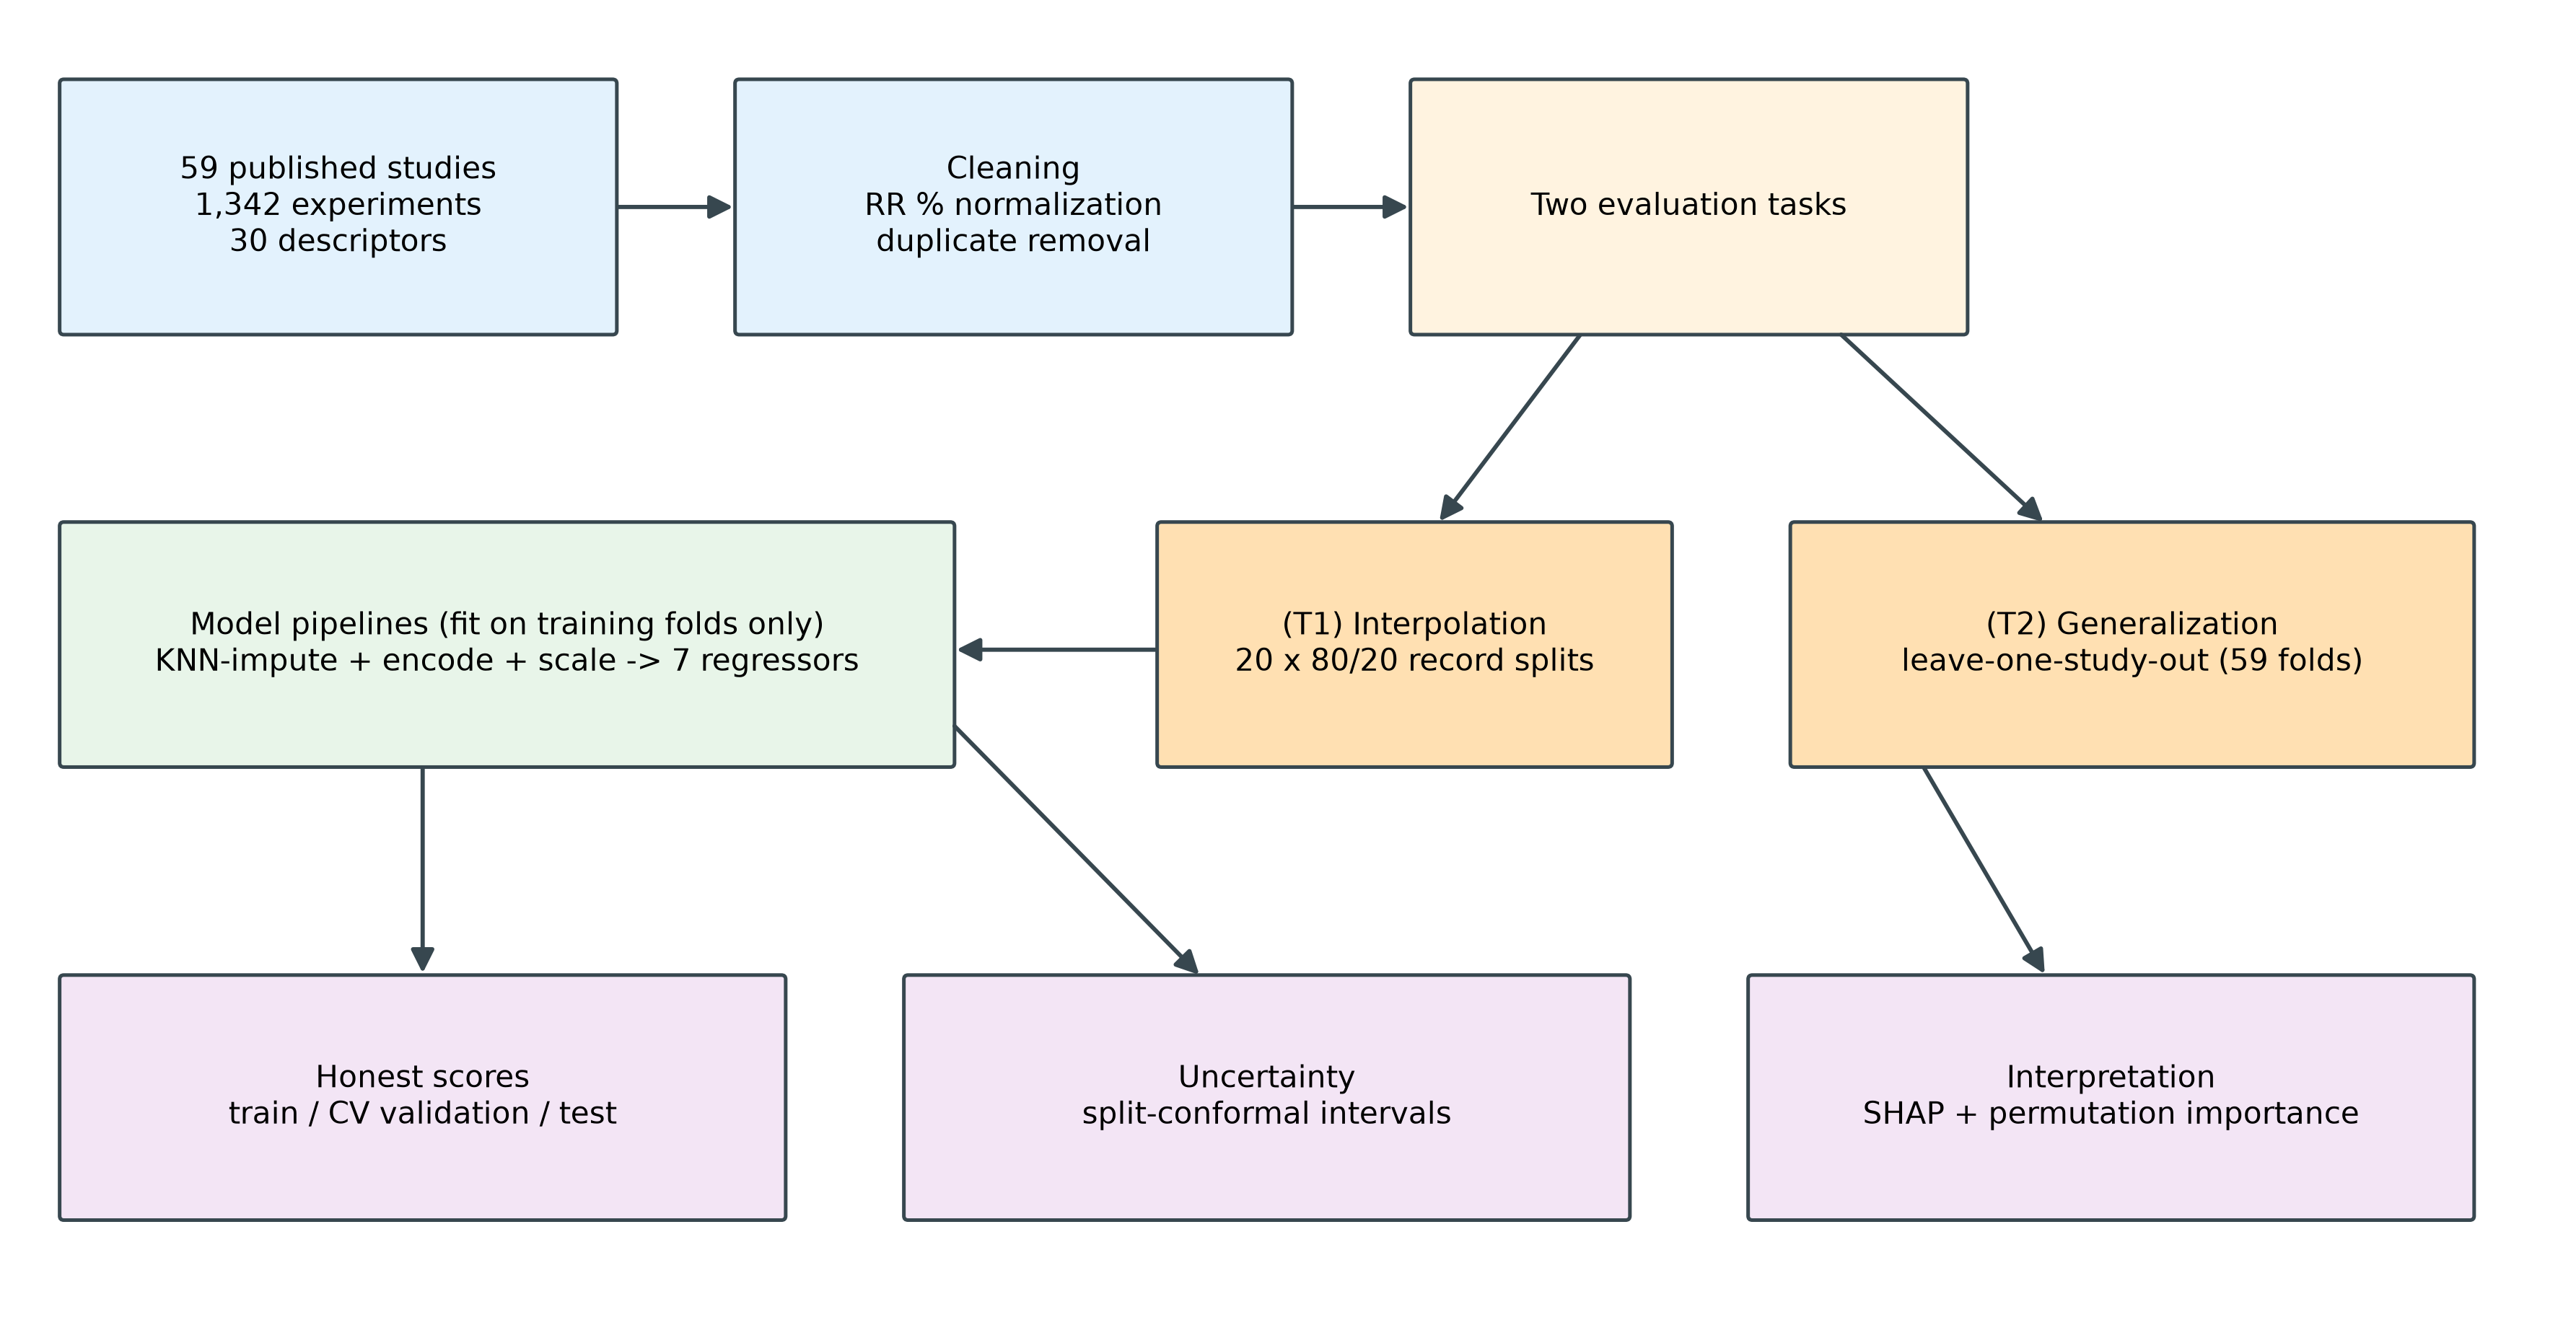
\includegraphics[width=\linewidth]{fig_workflow}
\caption{Evaluation workflow}
\label{fig:workflow}
\end{figure}

\subsection{Data curation}
\label{sec:data}

We compiled 1,342 batch-adsorption experiments for LDH--micropollutant
systems from 59 peer-reviewed studies. Each record holds 30 descriptors in
four groups: micropollutant properties (compound identity, log
$K_{\mathrm{ow}}$, molecular weight, the Abraham solvation parameters
$E$, $S$, $A$, $B$, $V$, and topological polar surface area), LDH
composition and synthesis (divalent and trivalent metal, molar ratio,
synthesis route, hydrothermal temperature and time, calcination
conditions, and composition-averaged elemental descriptors), material
texture (interlayer spacing $d_{003}$, BET surface area, pore volume,
average pore diameter, and point of zero charge pH$_{\mathrm{pzc}}$), and
operating conditions (pH, temperature, contact time, adsorbent dose, and
initial concentration). Table~\ref{tab:stats} summarizes the numeric
descriptors; the prediction target is the removal ratio (RR\%).

\textbf{Cleaning.} Values stored as fractions were converted to percent by
a range-aware rule that leaves already-percent data untouched, and
category labels were normalized (e.g., merging spelling variants of
\emph{co-precipitation}). Records identical in every descriptor were
reduced to a single occurrence, since duplicates spanning a train--test
boundary would let the test be answered by lookup; deduplication removed
83 records. Missing texture values were imputed by a
$k$-nearest-neighbor imputer computed in standardized space and mapped
back to physical units; the imputer, like every fitted transform in this
work, was trained on training folds only. The source study of each
record is retained as a grouping key and is never used as a model input.
Details of the cleaning rules are in Text~S1.

\begin{table}[t]
\centering
\caption{Summary statistics of the numeric descriptors}
\label{tab:stats}
\begin{tabular}{lccc}
\toprule
Descriptor & Median & Range & Missing (\%) \\
\midrule
\multicolumn{4}{l}{\emph{Micropollutant}} \\
log $K_{\mathrm{ow}}$ & $-0.02$ & $-2.67$--$4.51$ & 0 \\
MW (g/mol) & 331 & 152--734 & 0 \\
$E$ / $S$ / $A$ / $B$ / $V$ & 1.81 / 2.10 / 0.70 / 1.70 / 2.30 & -- & 0 \\
TPSA (\AA$^2$) & 76.2 & 37.3--194.0 & 0 \\
\midrule
\multicolumn{4}{l}{\emph{Composition and synthesis}} \\
M(II)/M(III) ratio & 3.0 & 0.5--8.0 & 0 \\
Avg.\ atomic weight (g/mol) & 48.1 & 24.8--73.7 & 0 \\
Avg.\ d-electrons & 4.25 & 0--8.89 & 0 \\
Avg.\ Pauling electronegativity & 1.59 & 1.30--1.89 & 0 \\
Hydrothermal temp.\ (\textcelsius) & 70 & 25--160 & 13.3 \\
Hydrothermal time (h) & 24 & 12--40 & 13.3 \\
Calcination temp.\ (\textcelsius) & 400 & 200--550 & 65.9 \\
Calcination time (h) & 4 & 1--12 & 65.9 \\
\midrule
\multicolumn{4}{l}{\emph{Material texture}} \\
$d_{003}$ (nm) & 0.77 & 0.25--1.13 & 2.5 \\
BET (m$^2$/g) & 82.0 & 0.4--225.7 & 7.9 \\
PV (cm$^3$/g) & 0.10 & 0--1.46 & 25.3 \\
APD (nm) & 8.4 & 0.2--64.2 & 13.9 \\
pH$_{\mathrm{pzc}}$ & 7.5 & 5.5--11.6 & 24.6 \\
\midrule
\multicolumn{4}{l}{\emph{Operating conditions}} \\
pH & 6.7 & 2.0--12.0 & 0 \\
Temperature (\textcelsius) & 25 & 10--55 & 0 \\
Contact time (h) & 1.5 & 0.02--192 & 0 \\
Dose (g/L) & 0.9 & 0.01--50 & 0 \\
$C_i$ (mg/L) & 40 & 1--1688 & 0 \\
\bottomrule
\end{tabular}
\end{table}

\subsection{Evaluation protocol}
\label{sec:protocol}

\textbf{Two prediction tasks.} We evaluate every model under two
protocols that correspond to the two services expected from
literature-trained models. Task (T1), \emph{within-system interpolation},
asks how well a model predicts RR\% for a studied
adsorbent--pollutant system at new operating conditions. Task (T2),
\emph{cross-study generalization}, asks how well the model predicts
systems it has never seen. Intuitively, (T1) allows the model to have
seen the material and the pollutant at other conditions, while (T2) does
not.

\textbf{Repeated splits for (T1).} A single random split can be lucky or
unlucky, so (T1) is measured over 20 seeded 80/20 record-level splits of
the duplicate-free data, and scores are reported as mean $\pm$ standard
deviation across repeats. Hyperparameters are tuned once (Section
\ref{sec:models}) and held fixed across repeats, so the spread reflects
sampling variability rather than tuning noise.

\textbf{Leave-one-study-out audit for (T2).} Each of the 59 studies $s$
is held out once; the model $f_{-s}$ is refit on the remaining 58
studies with fixed hyperparameters and scored on the held-out records:
\begin{equation}
\mathrm{MAE}_s \;=\; \frac{1}{n_s}\sum_{i \in s}
\bigl|\, y_i - f_{-s}(\mathbf{x}_i) \,\bigr| .
\label{eq:loso}
\end{equation}
Reporting the distribution of $\mathrm{MAE}_s$ across studies, rather
than one pooled score, exposes which systems transfer and which do not.
A learning curve over the number of training studies tests whether
cross-study error is limited by data volume or by data diversity.

\textbf{Naive baselines.} To make the error magnitudes interpretable, we
score three predictors that use no descriptors: the global training-mean;
the per-pollutant mean (the average RR\% of the same compound in the
training data, falling back to the global mean for unseen compounds); and,
for (T1) only, the per-study mean. A model is useful for screening only
if it beats these lookups on unseen studies.

\textbf{Leakage control.} Imputation, scaling, and categorical encoding
are embedded in each model pipeline and fitted on training folds only.
Hyperparameter tuning uses cross-validation folds that differ from the
folds used for reporting, and grouped tasks use group-aware folds
throughout. These controls address the leakage mechanisms documented for
applied ML \citep{kapoor2023leakage}, which we found to inflate reported
skill substantially when absent (Section~\ref{sec:rq2}).

\textbf{Deployment workflow.} The protocol doubles as a reusable recipe
for future compilations (Fig.~\ref{fig:workflow}). Step~1: curate and
normalize the literature records, retaining the source-study identifier.
Step~2: remove exact duplicates and declare the prediction task:
interpolation within studied systems or screening of new ones.
Step~3: split accordingly (record-level for the former, study-grouped
for the latter) and fit pipelines whose preprocessing sees training
folds only. Step~4: wrap the chosen model in split-conformal
calibration matched to the declared task and report coverage
empirically. Every step is implemented in the released pipeline
(\texttt{ldh\_pipeline.py}), so re-running the audit on an extended
compilation requires only the new spreadsheet.

\subsection{Regression models}
\label{sec:models}

We compare seven regressors spanning the model families used in the
adsorption-ML literature, chosen so that their inductive biases differ.
Throughout, $\mathbf{x}_i \in \mathbb{R}^{p}$ denotes the preprocessed
descriptor vector of record $i$ and $\hat{y}_i$ its predicted RR\%.

\textbf{Linear regression (LR)} fits one additive coefficient per
descriptor,
\begin{equation}
\hat{y} = \beta_0 + \sum_{j=1}^{p} \beta_j x_j ,
\label{eq:lr}
\end{equation}
with $\boldsymbol{\beta}$ estimated by least squares. It serves as the
interpretable floor: any nonlinearity or interaction in the adsorption
response appears as a gap between LR and the flexible models.

\textbf{$k$-nearest neighbors (KNN)} predicts the average target of the
$k$ closest training records in standardized feature space
\citep{cover1967knn},
\begin{equation}
\hat{y}(\mathbf{x}) = \frac{1}{k}\sum_{i \in \mathcal{N}_k(\mathbf{x})} y_i ,
\label{eq:knn}
\end{equation}
where $\mathcal{N}_k(\mathbf{x})$ holds the $k$ nearest neighbors under
Euclidean distance and $k$ is grid-searched between 1 and 9. KNN has no
functional form at all; its performance measures how far pure similarity
lookup carries prediction, which makes it a diagnostic for
near-duplicate structure in the data.

\textbf{Artificial neural network (ANN)} is a single-hidden-layer
perceptron trained by Adam \citep{rumelhart1986backprop},
\begin{equation}
\hat{y} = \mathbf{w}^{\top} \sigma\!\left(W\mathbf{x} + \mathbf{b}\right) + b_0 ,
\label{eq:ann}
\end{equation}
with 32 hidden units and rectified-linear activation
$\sigma(z) = \max(0, z)$, matching the compact architectures used in
prior adsorption studies. Larger architectures were not explored because
the dataset holds fewer than $10^3$ effective degrees of freedom per
feature.

\textbf{Cubist} builds a set of rules $R_m$ whose leaves hold linear
models \citep{quinlan1992m5},
\begin{equation}
\hat{y}(\mathbf{x}) = \operatorname*{avg}_{m:\,\mathbf{x} \in R_m}
\Bigl( \beta_{0}^{(m)} + \textstyle\sum_j \beta_{j}^{(m)} x_j \Bigr),
\label{eq:cubist}
\end{equation}
optionally smoothed toward the targets of nearby training instances;
committees and neighbors are grid-searched. Unlike constant-leaf trees,
its leaf-linear structure can extrapolate moderately beyond the training
range of a rule, a property that becomes relevant under (T2).

\textbf{Random forest (RF)} averages $B$ decorrelated trees grown on
bootstrap samples \citep{breiman2001rf},
\begin{equation}
\hat{y}(\mathbf{x}) = \frac{1}{B}\sum_{b=1}^{B} T_b(\mathbf{x}),
\label{eq:rf}
\end{equation}
providing a variance-reduced piecewise-constant baseline among the
ensembles.

\textbf{Gradient-boosted trees} build the prediction stagewise, each new
tree fitting the residual structure left by its predecessors,
\begin{equation}
F_m(\mathbf{x}) = F_{m-1}(\mathbf{x}) + \nu\, h_m(\mathbf{x}),
\label{eq:gb}
\end{equation}
with learning rate $\nu$ and base trees $h_m$. \textbf{XGBoost}
implements Eq.~(\ref{eq:gb}) with second-order updates and a regularized
objective that penalizes the number of leaves and their weights
\citep{chen2016xgboost}; \textbf{histogram gradient boosting (HistGB)}
is the scikit-learn implementation with histogram-binned split finding
\citep{ke2017lightgbm, pedregosa2011sklearn}. Both are the strongest
current defaults for tabular data.

Tree-ensemble hyperparameters were tuned with the TPE sampler of Optuna
over 30 trials \citep{akiba2019optuna} on cross-validation folds of the
training data. Scale-sensitive models (LR, KNN, ANN, Cubist) receive a
standardizer inside their pipeline; tree ensembles operate on raw feature
scales. Search spaces and selected values are in Table~S1; all splits,
folds, and samplers are seeded for reproducibility.

\subsection{Feature screening and selection}
\label{sec:screening}

Multicollinearity is diagnosed with the variance inflation factor,
\begin{equation}
\mathrm{VIF}_j = \frac{1}{1 - R_j^{2}},
\label{eq:vif}
\end{equation}
where $R_j^{2}$ is the coefficient of determination of descriptor $j$
regressed on all other descriptors (targets excluded). Because
descriptors are constant within a study, the study-cluster structure
drives VIF values orders of magnitude beyond the usual threshold of 10
(Section~\ref{sec:eda}), so VIF is used here as a redundancy diagnostic
rather than an automatic elimination rule.

Feature selection is then evaluated the same way as the models
themselves: three nested descriptor sets (the full set of 30, a
correlation-screened set of 21 that drops the collinear Abraham and
composition-averaged block, and the 10 descriptors with the best median
permutation-importance rank) are compared under both tasks with fixed
hyperparameters. Judging a feature set only under (T1) would inherit
the same optimism as judging a model there, so both tasks are reported.

\subsection{Uncertainty and applicability domain}
\label{sec:uq}

\textbf{Split-conformal intervals.} We wrap the best model in
split-conformal prediction \citep{vovk2005conformal, lei2018conformal}.
A calibration subset of $n$ records is withheld from training, absolute
residuals $r_i = |y_i - \hat{y}_i|$ are computed on it, and the interval
half-width is their conformal quantile
\begin{equation}
q \;=\; \mathrm{Quantile}\!\left(\{r_i\}_{i=1}^{n};\;
\frac{\lceil (n+1)(1-\alpha) \rceil}{n}\right),
\label{eq:conformal}
\end{equation}
so that each test prediction is reported as $[\hat{y}-q,\ \hat{y}+q]$
with nominal coverage $1-\alpha = 0.9$. For task (T2) the calibration
subset is drawn as whole studies, so the calibration residuals reflect
the new-study setting. Conformal validity assumes exchangeability
between calibration and test units, which grouped data satisfy only
approximately; we therefore report empirical coverage for both tasks
rather than assuming it.

\textbf{Applicability domain.} As a candidate trust flag we compute, for
each test record, the mean standardized distance to its five nearest
training records in the preprocessed feature space. Records far from the
training distribution should receive predictions with caution; we
validate the flag by correlating it with realized absolute error rather
than assuming it works.

\subsection{Feature engineering and attribution}
\label{sec:features}

Beyond the raw descriptors, we construct three features with mechanistic
meaning: the electrostatic driving force pH$-$pH$_{\mathrm{pzc}}$, whose
sign determines whether the LDH surface is positively or negatively
charged relative to the solution; the initial loading ratio $C_i$/dose;
and the interaction log $K_{\mathrm{ow}} \times$
(pH$-$pH$_{\mathrm{pzc}}$) coupling hydrophobicity with surface charge.
Both tasks are re-evaluated with and without these features. Feature
attributions are computed with SHAP \citep{lundberg2017shap} on the
held-out test set using the fitted models, complemented by permutation
importance ranks across all seven models and one-dimensional partial
dependence profiles, and the resulting patterns are read against the
expected electrostatic and hydrophobic mechanisms.

\subsection{Performance metrics}
\label{sec:metrics}

Model skill is reported as the coefficient of determination,
\begin{equation}
R^2 = 1 - \frac{\sum_i (y_i - \hat{y}_i)^2}{\sum_i (y_i - \bar{y})^2},
\label{eq:r2}
\end{equation}
the root mean square error,
$\mathrm{RMSE} = \smash{\sqrt{\tfrac{1}{n}\sum_i (y_i - \hat{y}_i)^2}}$,
and the mean absolute error,
$\mathrm{MAE} = \tfrac{1}{n}\sum_i |y_i - \hat{y}_i|$,
each computed on three bases with distinct meanings: the training
records (in-sample fit), cross-validation folds of the training set
(validation), and the held-out test records of the task at hand. All
three are reported to keep the in-sample ceiling and the generalization
estimate visibly separate. Wall-clock training and prediction times are
reported in Section~\ref{sec:timing}.

\section{Results and discussion}
\label{sec:results}

Section~\ref{sec:eda} first characterizes the compiled dataset. The
modeling experiments then answer four research questions. (RQ1)~How
accurately do the models predict RR\% for studied systems at new
operating conditions? (RQ2)~Does this accuracy transfer to systems from
unseen studies? (RQ3)~Can the uncertainty of individual predictions be
quantified reliably under both tasks? (RQ4)~Which factors govern the
predictions, and are they chemically plausible?

\subsection{Dataset characteristics}
\label{sec:eda}

Figure~\ref{fig:eda} summarizes the compiled data. Removal ratios span
the full 0--100\% range with a median above 50\%, but the distribution
differs strongly between pollutants and between LDH metal pairs
(Fig.~\ref{fig:eda}a,b), reflecting both genuine chemistry and the
uneven attention different systems have received in the literature. The
study-size distribution is heavily skewed: the largest single study
contributes 220 of the 1,342 records, the median study only 17, and a
random record-level sample is therefore dominated by a handful of
intensively measured systems. Spearman correlations among the numeric
descriptors (Fig.~S1) show the expected blocks: the Abraham solvation
parameters correlate strongly with molecular weight and with each other,
and the composition-averaged elemental descriptors correlate with the
metal identities they are derived from. This redundancy motivates the
correlated-descriptor experiment in Section~S3 and, more fundamentally,
explains why record-level splits leak: within one study, most descriptor
columns are constant, so any two records of the same study are
near-duplicates in feature space. Missingness is confined to the
synthesis and texture blocks (Table~\ref{tab:stats}): calcination
conditions are unreported for two thirds of the records, and
pH$_{\mathrm{pzc}}$ and pore volume for roughly a quarter, which is why
imputation quality matters and why texture-based mechanistic claims from
compiled data warrant caution.

\begin{figure}[t]
\centering
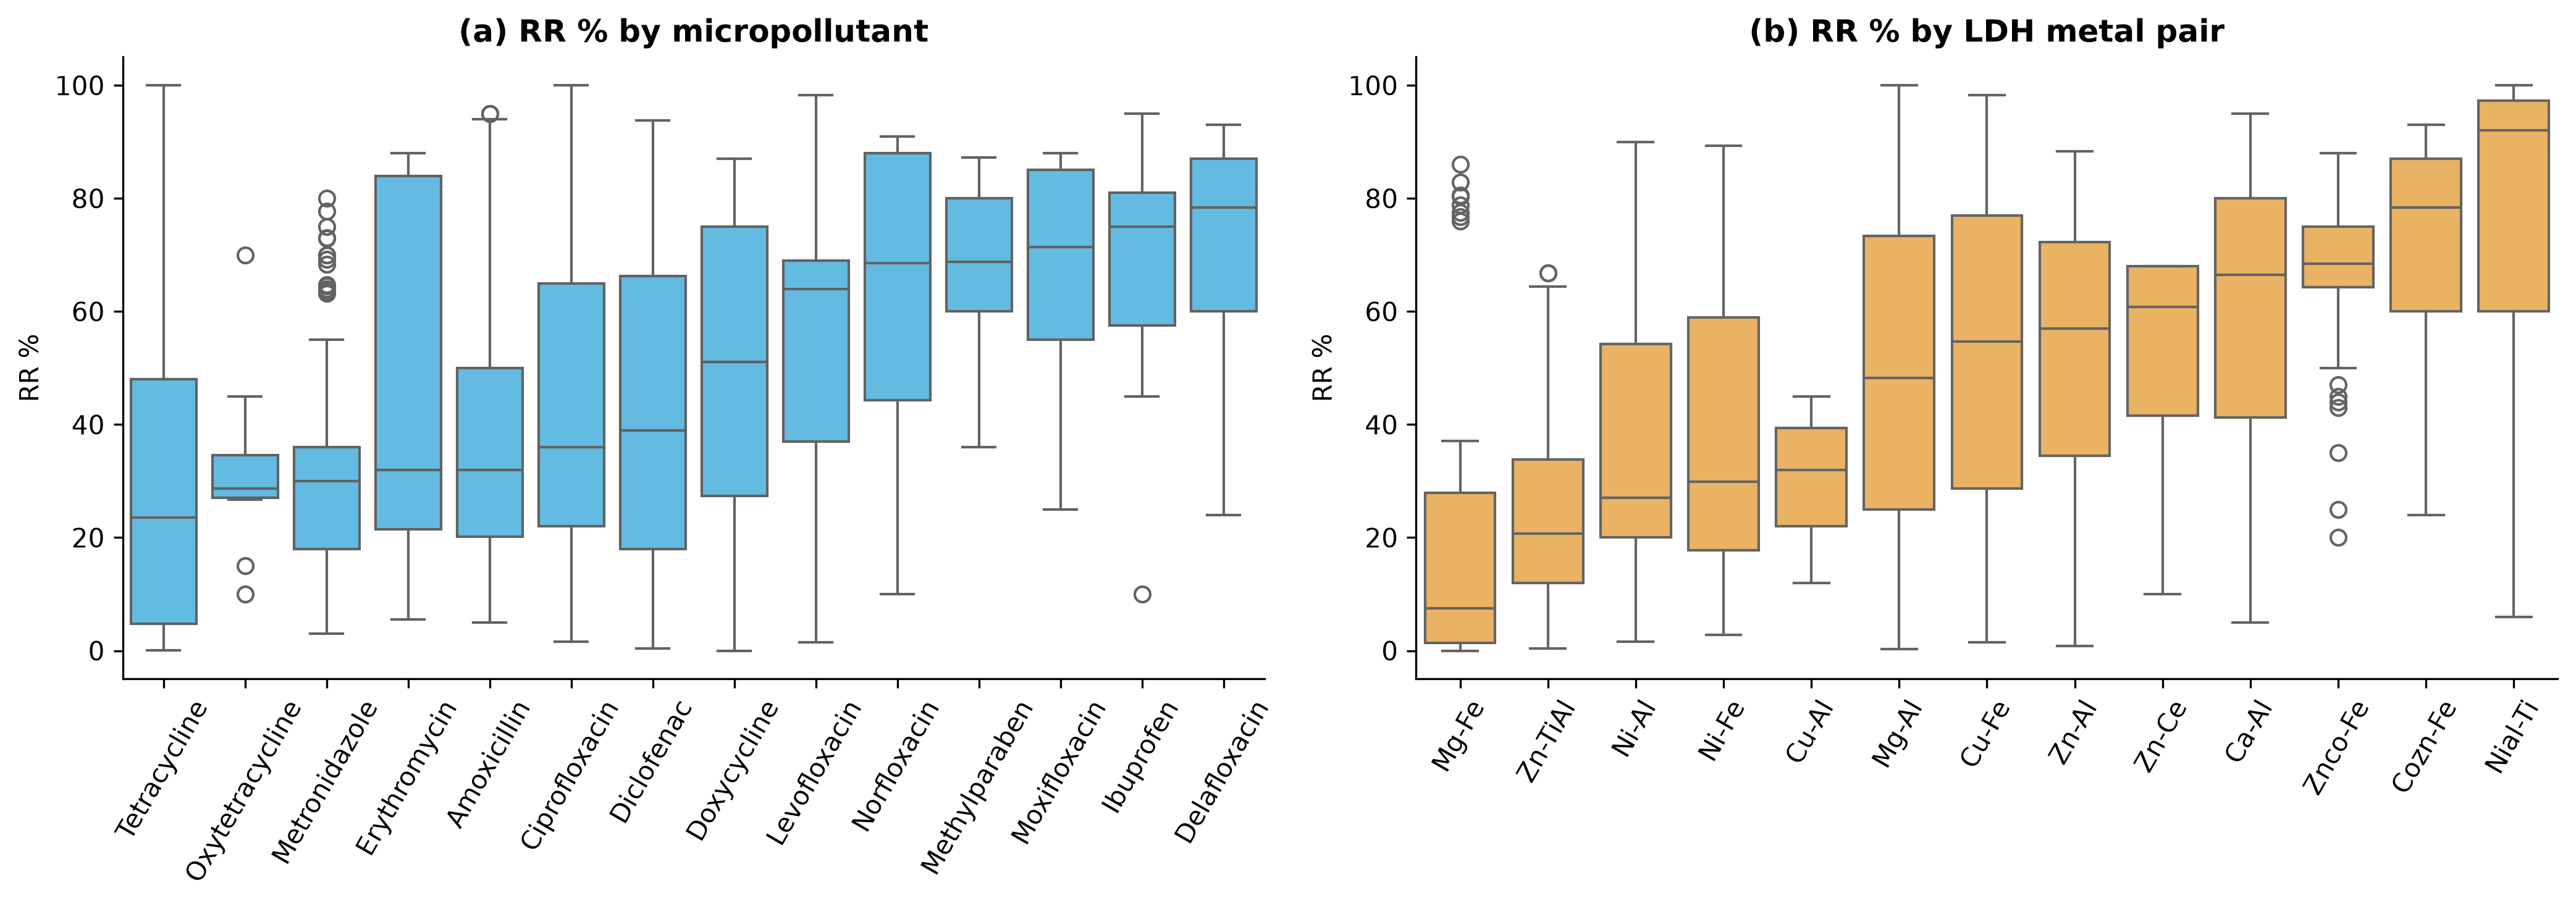
\includegraphics[width=\linewidth]{fig_eda_rr}
\caption{Removal-ratio distributions by pollutant and by metal pair}
\label{fig:eda}
\end{figure}

\subsection{Within-system interpolation (RQ1)}
\label{sec:rq1}

Table~\ref{tab:interp} answers (RQ1) by comparing the seven models and
the naive baselines under task (T1), reported as mean $\pm$ SD over 20
seeded splits. The tree ensembles lead: XGBoost and HistGB reach test
$R^2$ of $0.84$--$0.85$ with RMSE near 11 percentage points, followed by
Cubist and RF, while LR trails far behind. This is because RR\%
responds nonlinearly to the operating conditions, with thresholds in pH
and dose that additive linear terms cannot represent. The baselines put
these numbers in perspective. The per-study mean, which uses no
descriptors at all, already attains $R^2$ of $0.43$ (MAE 16.7): nearly
half of the variance a record-level split appears to explain is
available from system identity alone, and LR barely improves on it. The
ensembles' further gain to $R^2$ of $0.85$ therefore reflects genuine
modeling of the operating conditions within known systems. The
in-sample $R^2$ of the ensembles approaches 0.99, and the gap to the
test score is the expected overfitting margin of high-capacity learners
rather than a protocol artifact; the cross-validation and test scores
agree closely. Figure~\ref{fig:parity} shows the parity and residual
plots of the best model on the reference split. It is worth noting that
these scores are already 2--3 RMSE points more conservative than a
protocol without duplicate removal on the same data, since deduplication
alone eliminates records whose test values could be looked up verbatim
from training.

\begin{table}[t]
\centering
\caption{Model and baseline performance under within-system
interpolation (T1), mean $\pm$ SD over 20 seeded 80/20 splits
[VALUES FROM repeated\_interp\_summary.csv]}
\label{tab:interp}
\begin{tabular}{lccc}
\toprule
Model & Test $R^2$ & Test MAE & Test RMSE \\
\midrule
XGBoost & $0.84 \pm 0.03$ & $6.3 \pm 0.6$ & $11.1 \pm 1.0$ \\
HistGB  & $0.85 \pm 0.03$ & $6.3 \pm 0.5$ & $10.8 \pm 1.0$ \\
KNN     & $0.73 \pm 0.06$ & $7.8 \pm 0.8$ & $14.4 \pm 1.5$ \\
Cubist  & $0.79 \pm 0.03$ & $8.0 \pm 0.6$ & $12.7 \pm 1.0$ \\
RF      & $0.78 \pm 0.03$ & $8.6 \pm 0.5$ & $13.0 \pm 0.9$ \\
ANN     & $0.54 \pm 0.05$ & $14.4 \pm 0.7$ & $19.1 \pm 0.9$ \\
LR      & $0.40 \pm 0.04$ & $17.4 \pm 0.5$ & $21.7 \pm 0.7$ \\
\midrule
Per-study mean     & $0.43 \pm 0.05$ & $16.7 \pm 0.8$ & $21.2 \pm 0.9$ \\
Per-pollutant mean & $0.18 \pm 0.03$ & $21.4 \pm 0.6$ & $25.4 \pm 0.6$ \\
Global mean        & $-0.01 \pm 0.01$ & $24.9 \pm 0.7$ & $28.1 \pm 0.6$ \\
\bottomrule
\end{tabular}
\end{table}

\subsection{Cross-study generalization (RQ2)}
\label{sec:rq2}

Figure~\ref{fig:loso} answers (RQ2) with the leave-one-study-out audit.
The picture changes sharply: the median per-study MAE of the best models
rises to 14--16 percentage points, two to three times their
interpolation error, and the per-study $R^2$ is positive for only 4 of
the 32 studies large enough to evaluate it. This is because the models
exploit descriptor combinations that identify a material--pollutant
system rather than transferable structure--activity relations; when all
records of a system are withheld, that shortcut disappears. The
baseline comparison adds an important nuance. Descriptor-free lookups
transfer even worse: the global training-mean reaches a median per-study
MAE of 24 points and the per-pollutant mean of 25, so the models do
reduce the naive error by roughly 40 percent, and Cubist beats the
per-pollutant lookup in 41 of the 59 studies. The models therefore
track the level differences between systems while failing to resolve the
condition response within an unseen system, which is exactly why the
per-study $R^2$ (measured against each study's own variance) stays
negative even as the MAE gain over the baselines is large. Screening
applications get a coarse ranking signal from these models, not
engineering precision. The
per-study distribution in Fig.~\ref{fig:loso}b is wide rather than
uniformly poor: for Cubist, 20 of the 59 studies are predicted with
errors comparable to the interpolation regime (MAE below 6 points),
while 9 studies exceed 30 points. Notably, the model ranking also
reorders: Cubist, mid-table under interpolation, attains the lowest
cross-study median, which could be explained by its rule-plus-linear
structure extrapolating more gracefully than deep tree ensembles.

\textbf{Which systems transfer.} Figure~\ref{fig:transfer} breaks the
per-study errors down by chemistry, and the pattern follows literature
density. Ciprofloxacin studies, which dominate the compilation (32 of
59 studies), are predicted with a median MAE of 5 points, and Zn--Al
systems (28 studies) with 5 points, because each held-out study of these
families leaves many close relatives in training. Sparsely covered
chemistries fare far worse: tetracycline, diclofenac, and levofloxacin
studies show median errors above 20 points, and Ni--Fe systems above 30.
Error also grows with the held-out study's own scope: per-study MAE
correlates with both the number of records and the within-study spread
of RR\% ($r \approx 0.45$ for each), meaning studies that explore wide
condition ranges are precisely the ones an outside model cannot resolve.
The learning curve in Fig.~\ref{fig:lc}b is flat between 5 and 40
training studies, suggesting that cross-study error is limited by the
diversity of compiled systems rather than by record count. This
supports our central argument that random-split scores, including those
in Table~\ref{tab:interp}, must not be read as screening skill: the same
models, the same data, and the same preprocessing yield near-zero skill
when the test set contains genuinely new systems.

\begin{figure}[t]
\centering
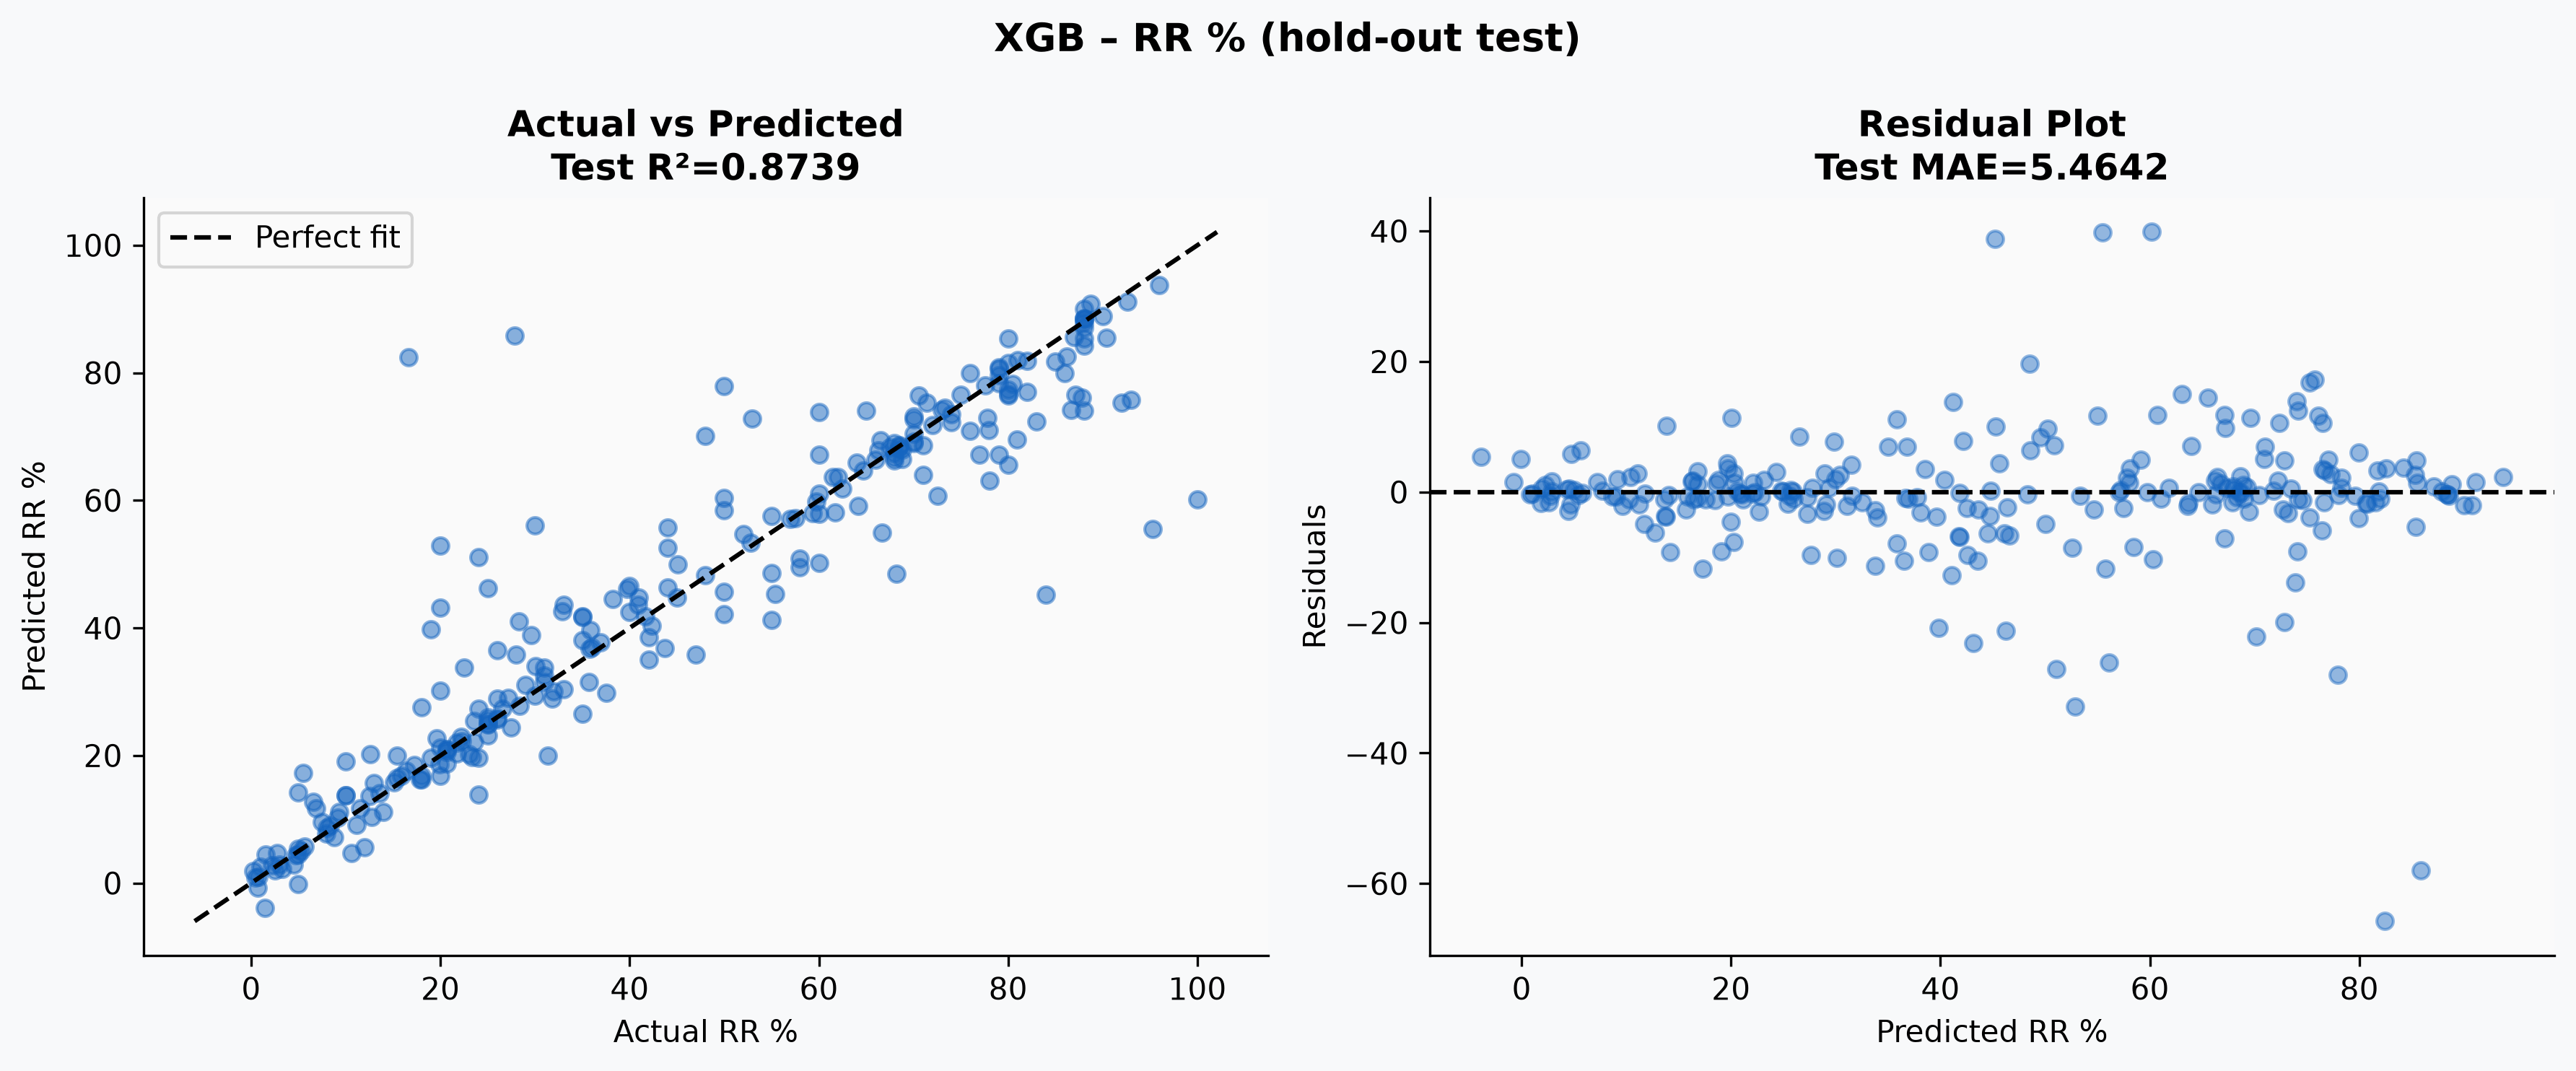
\includegraphics[width=\linewidth]{fig_parity}
\caption{Parity and residual plots of the best model under interpolation}
\label{fig:parity}
\end{figure}

\begin{figure}[t]
\centering
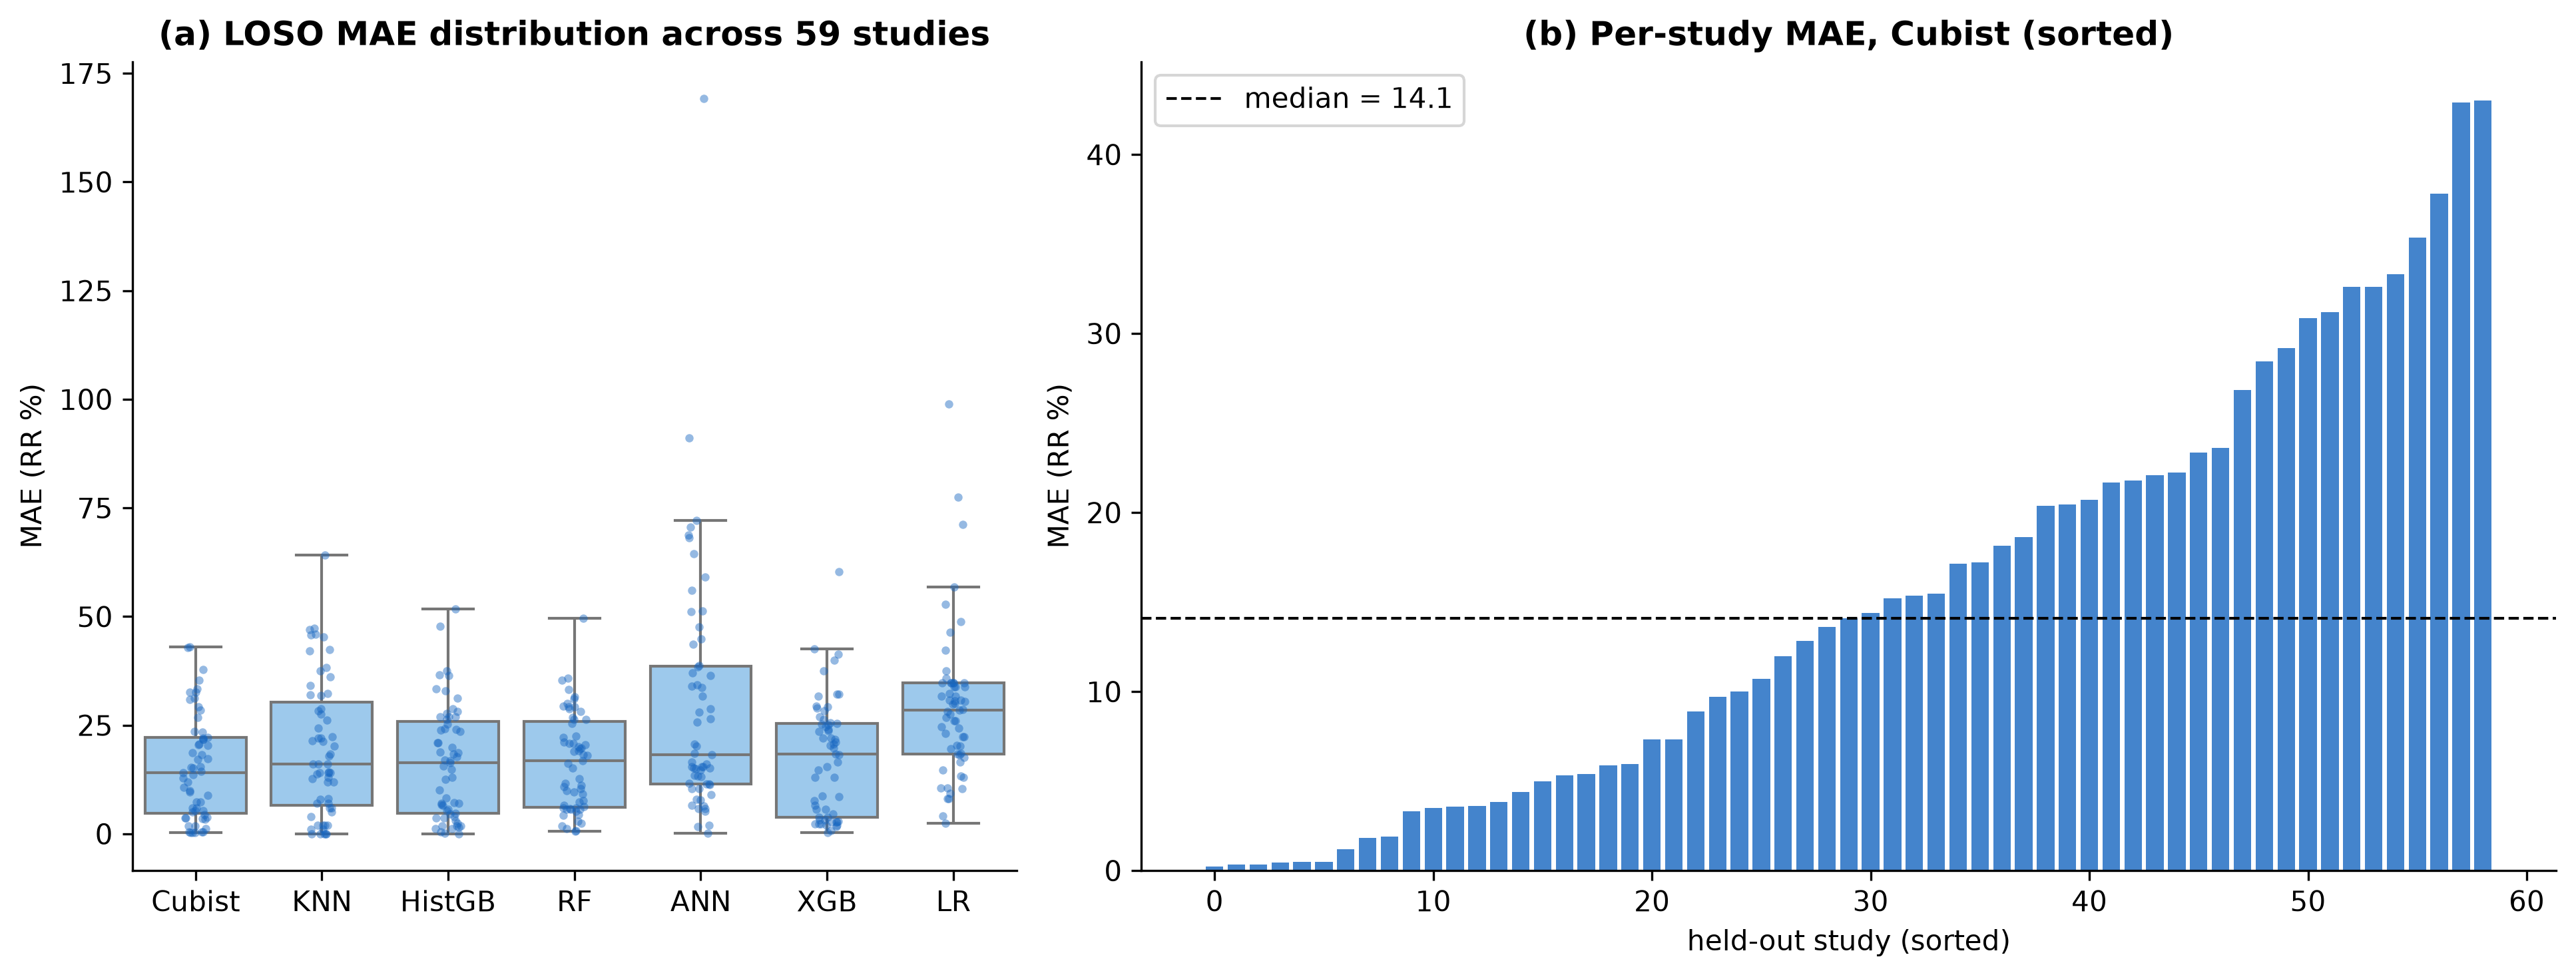
\includegraphics[width=\linewidth]{fig_loso_audit}
\caption{Leave-one-study-out audit across 59 studies}
\label{fig:loso}
\end{figure}

\begin{figure}[t]
\centering
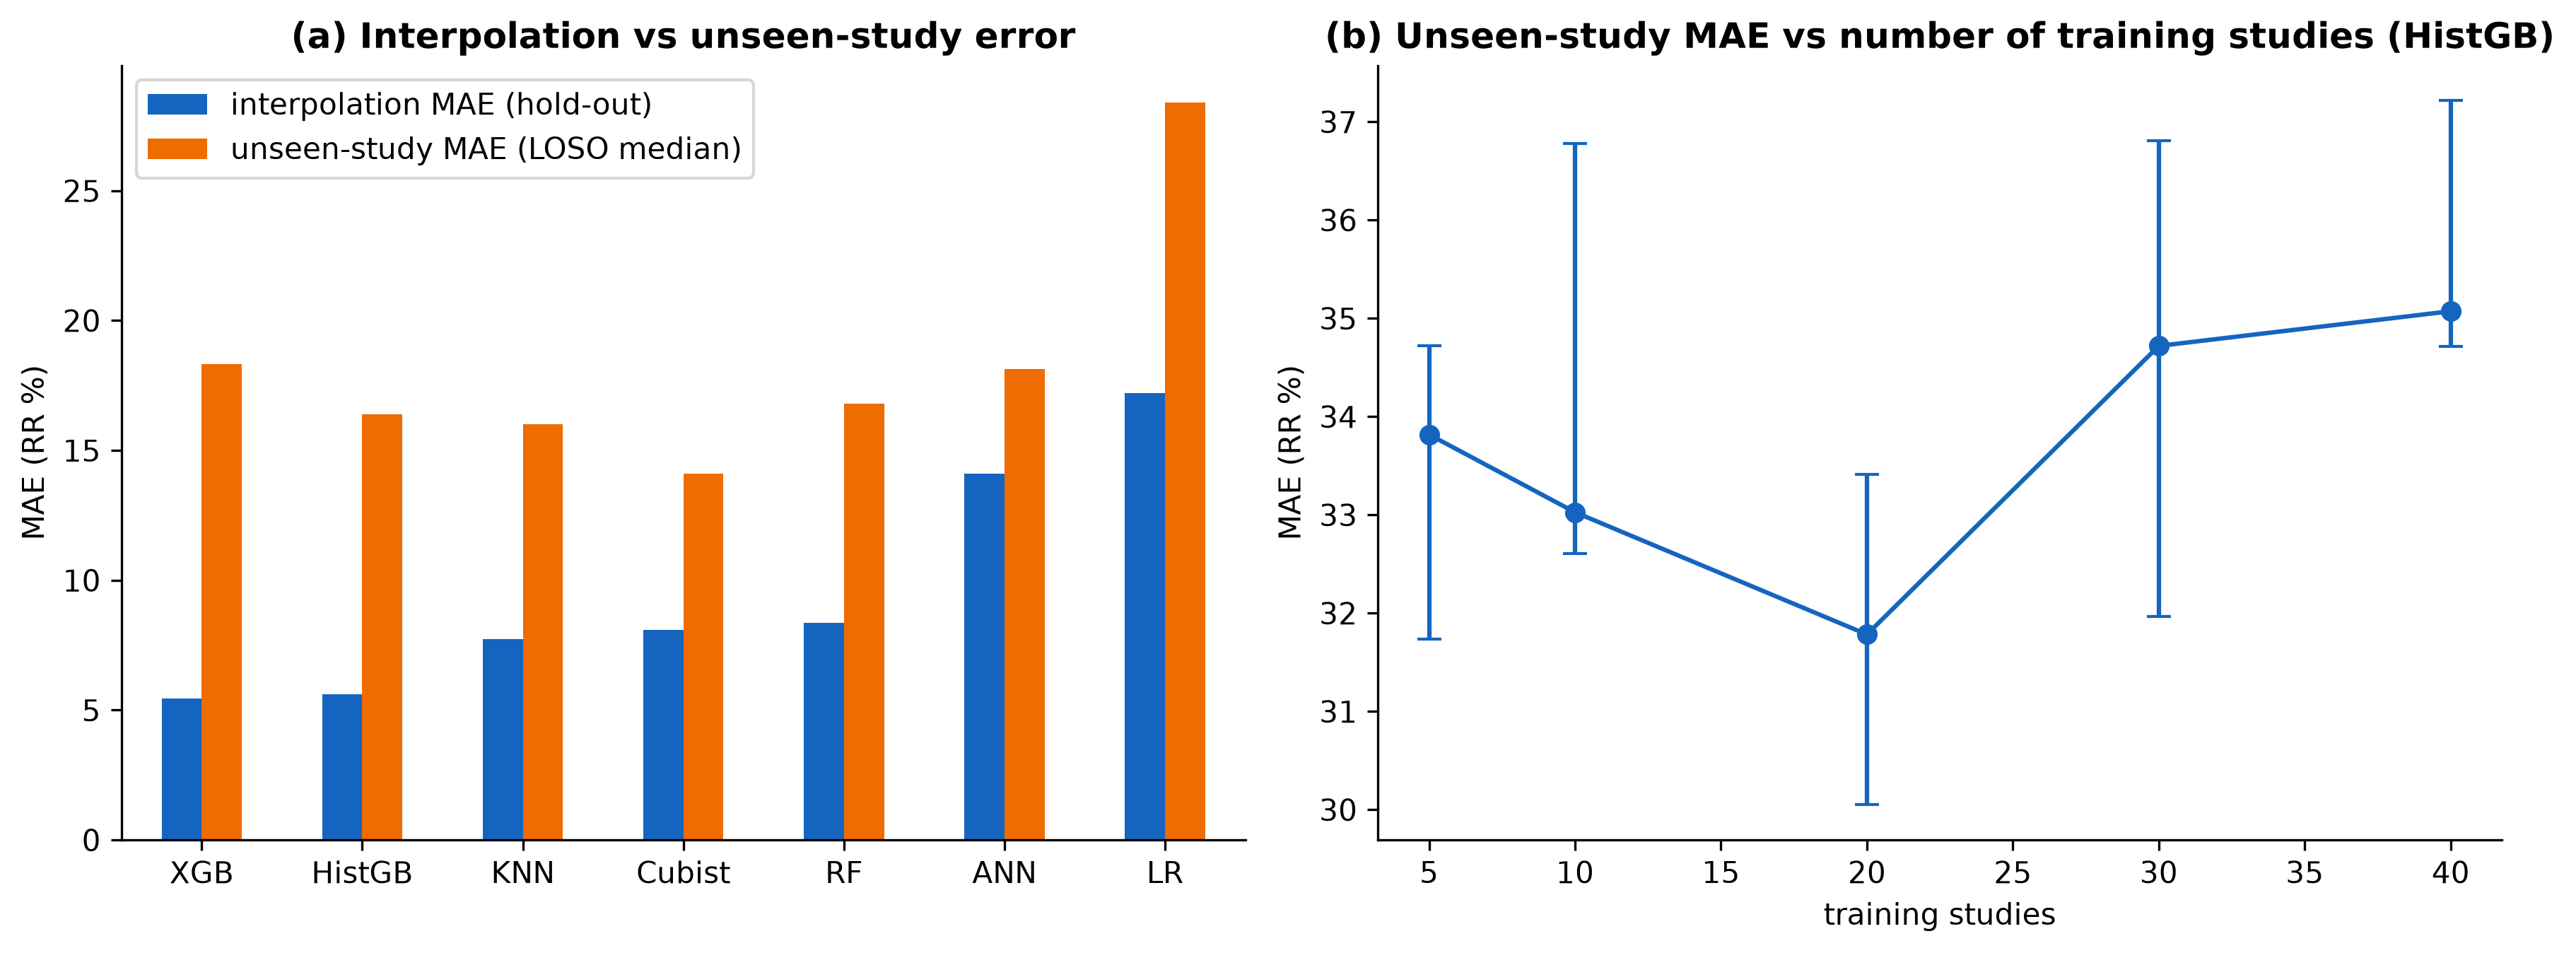
\includegraphics[width=\linewidth]{fig_learning_curve}
\caption{Interpolation versus unseen-study error and learning curve}
\label{fig:lc}
\end{figure}

\begin{figure}[t]
\centering
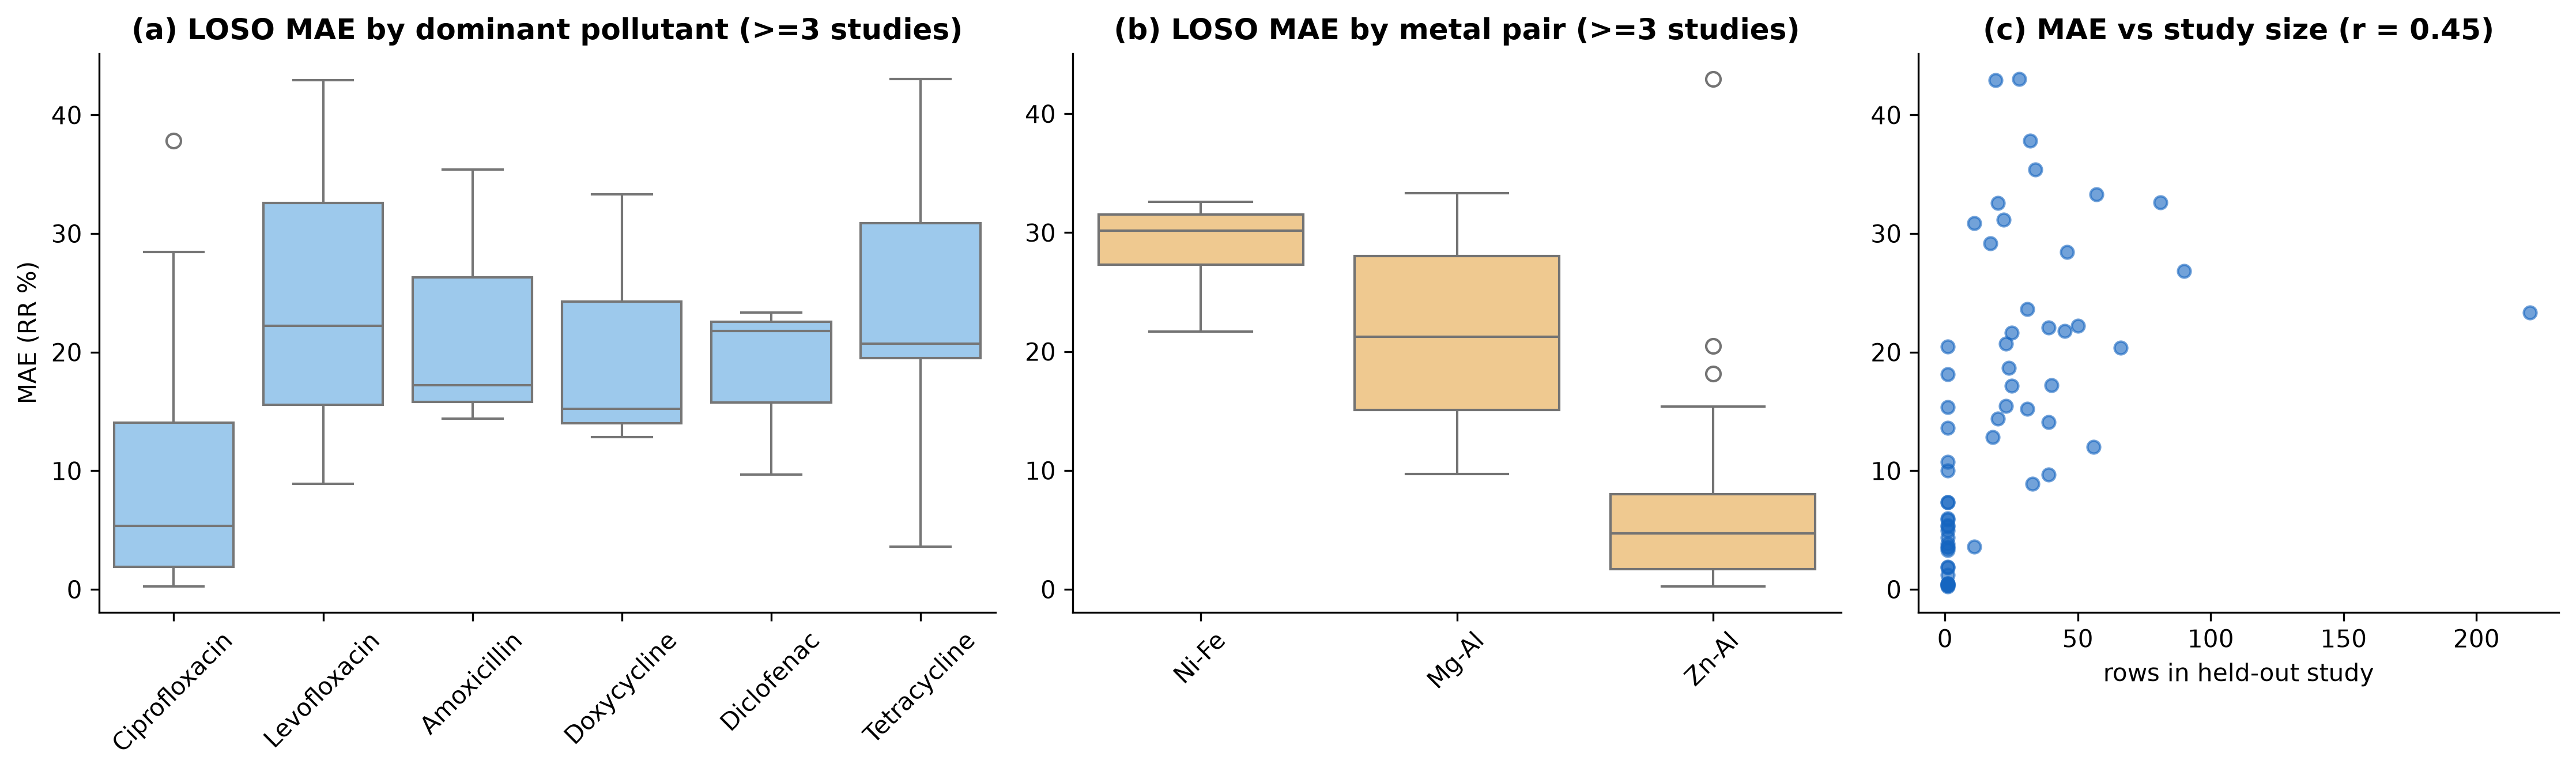
\includegraphics[width=\linewidth]{fig_transfer_breakdown}
\caption{Cross-study error by pollutant, metal pair, and study size}
\label{fig:transfer}
\end{figure}

\subsection{Uncertainty and applicability domain (RQ3)}
\label{sec:rq3}

Figure~\ref{fig:conformal} answers (RQ3). Under interpolation, the
split-conformal 90\% intervals of Eq.~(\ref{eq:conformal}) achieve
empirical coverage of 93\% with a half-width of 19 percentage points, so
predictions for studied systems can be certified at a practically useful
precision. Under the new-study task, coverage is maintained (99\%) only
because the study-grouped calibration inflates the half-width to 68
points, an interval spanning most of the 0--100 RR\% range and therefore
carrying little decision value. This is because residual magnitudes
differ systematically between systems, so a single global quantile must
cover the worst of them. The distance-based applicability-domain flag
does not compensate: the mean distance to the five nearest training
records carries essentially no information about realized error in
either task ($r \le 0.06$, Fig.~\ref{fig:conformal}b), although such
distance heuristics are widely used as trust flags. A key finding is
therefore that the uncertainty tools inherit the transfer problem
itself: interpolation predictions can be certified, whereas no
construction we tested produces informative guarantees for unseen
systems, and coverage claims must be validated empirically for the
deployment task.

\begin{figure}[t]
\centering
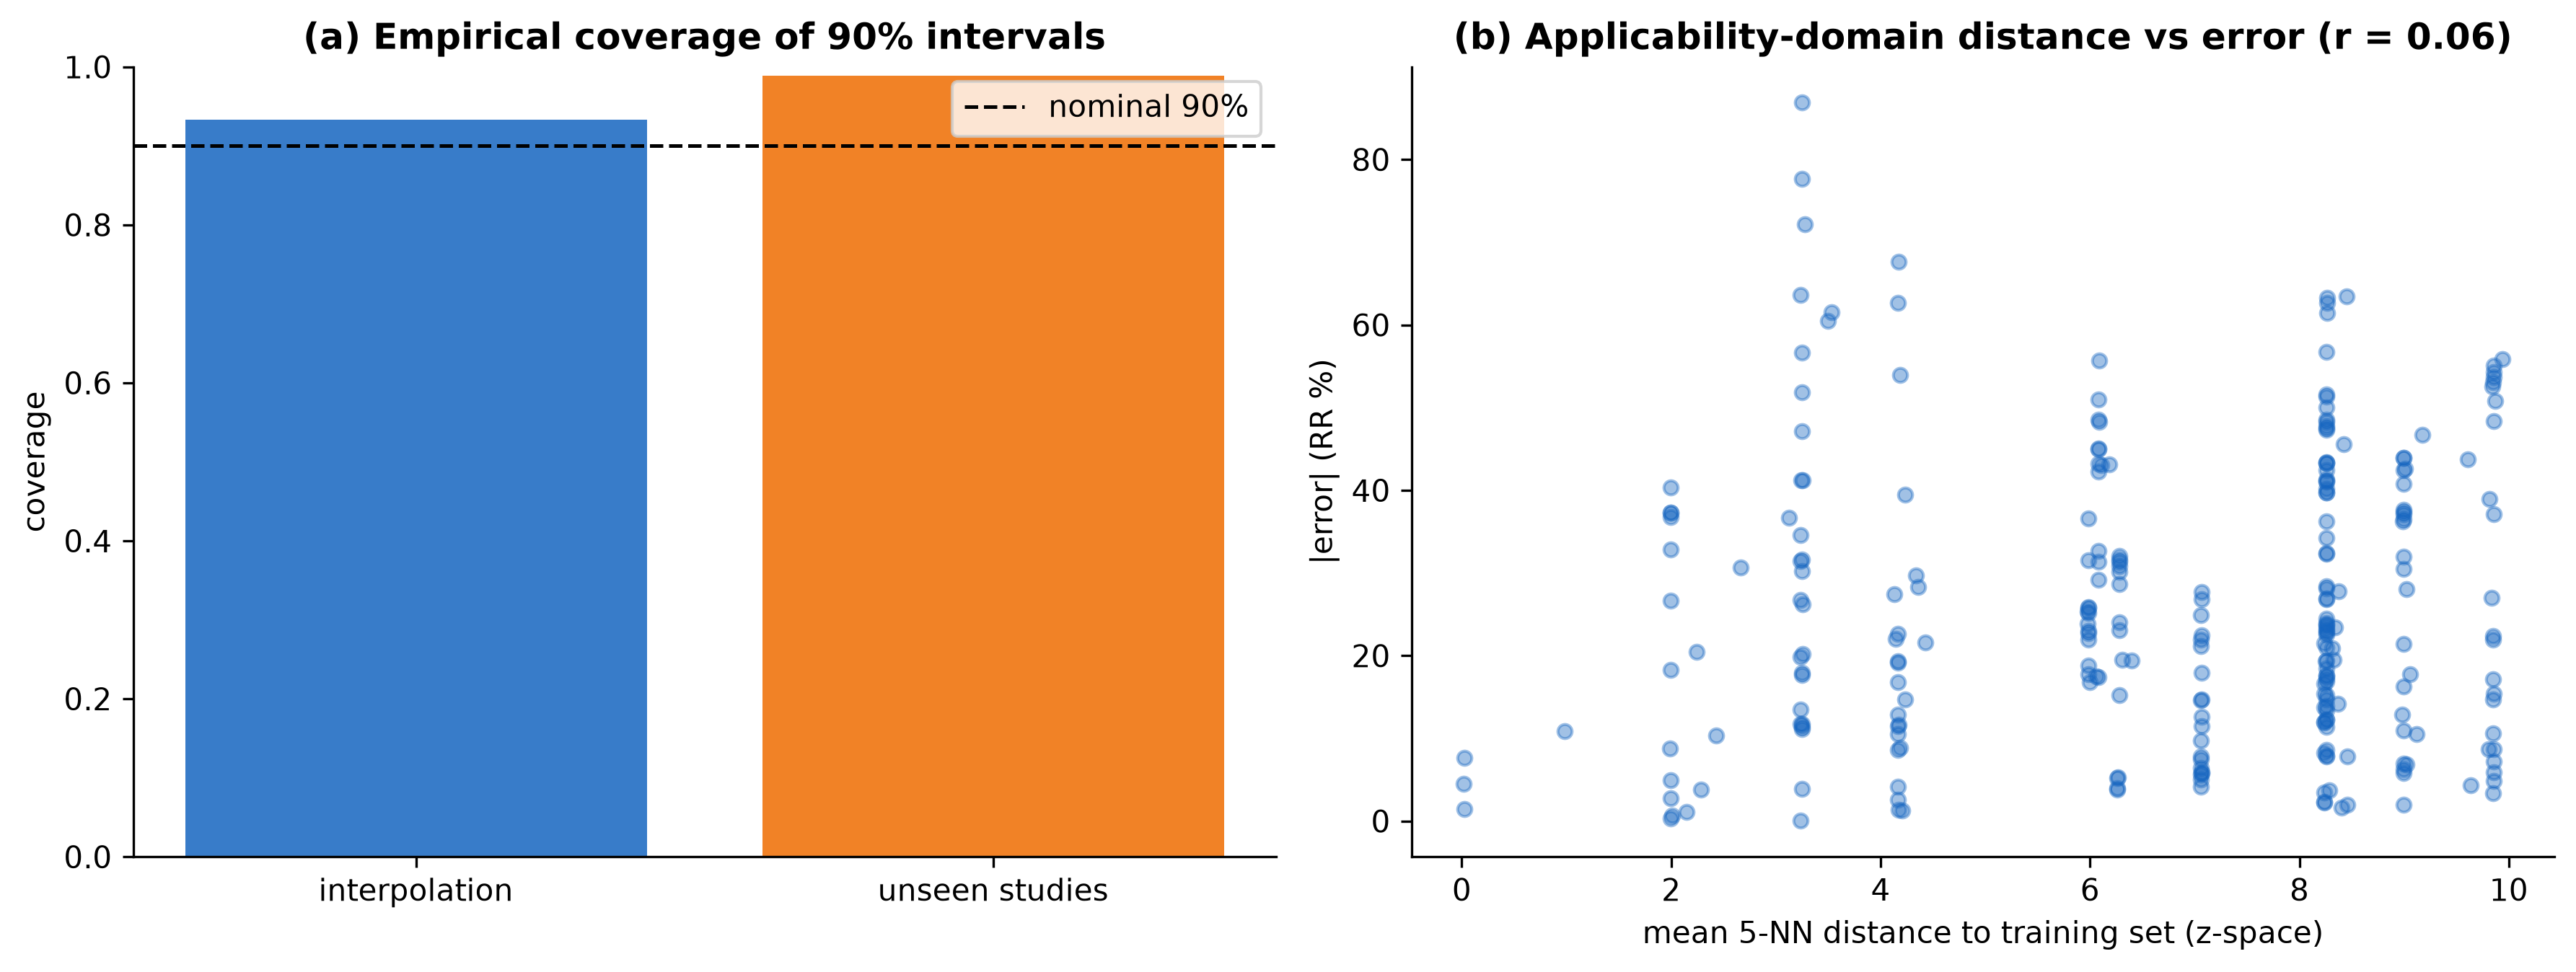
\includegraphics[width=\linewidth]{fig_conformal_ad}
\caption{Conformal coverage and applicability-domain flag}
\label{fig:conformal}
\end{figure}

\subsection{Feature effects and mechanistic reading (RQ4)}
\label{sec:rq4}

Figure~\ref{fig:shap} and Table~\ref{tab:ranks} answer (RQ4). Adding
the chemistry-informed features leaves both tasks essentially unchanged
(interpolation MAE 5.6 versus 5.8 points; cross-study median 16.4 versus
16.0), indicating that the models already reconstruct these combinations
internally from pH, pH$_{\mathrm{pzc}}$, and dose. Their value here is
interpretive rather than predictive.

\textbf{Operating conditions dominate.} Permutation-importance ranks on
the hold-out set (Table~\ref{tab:ranks}) agree across six of the seven
models on the leading factors: adsorbent dose ranks first, followed by
contact time, initial concentration, and pH, with the first material
property (BET) at median rank six and the first pollutant descriptor
(log $K_{\mathrm{ow}}$) at rank nine; only the additive LR deviates.
The partial-dependence profiles of the three leading features (Fig.~S2)
show textbook adsorption behavior: removal rises steeply with dose up to
roughly 2--5 g/L and then saturates, rises within the first hours of
contact and plateaus at equilibrium, and declines with initial
concentration beyond roughly 200 mg/L as fixed capacity is exhausted.
Within known systems, the models therefore learn genuine
condition--response physics. The same ranking, however, explains the
transfer failure of Section~\ref{sec:rq2} from a second direction:
material and pollutant descriptors, the only information available about
an unseen system, contribute comparatively little to the fitted models.

\textbf{Mechanistic reading.} The SHAP dependence of
pH$-$pH$_{\mathrm{pzc}}$ (Fig.~\ref{fig:shap}a) is not smoothly
monotone but threshold-like: contributions stay within a few points
while the surface remains positively charged, and a sharp penalty of up
to nine points appears once solution pH exceeds pH$_{\mathrm{pzc}}$ by
more than about three units. Coloring this dependence by log
$K_{\mathrm{ow}}$ (Fig.~S3) shows the penalty concentrated among
hydrophilic compounds, consistent with electrostatic repulsion of
anionic species from a negatively charged surface while hydrophobic
partitioning buffers the loss for lipophilic ones. Log
$K_{\mathrm{ow}}$ itself is the strongest chemical attribution
(Fig.~\ref{fig:shap}b), monotone from roughly $-5$ points for the most
hydrophilic compounds to $+15$ for the most lipophilic. BET surface
area (Fig.~\ref{fig:shap}c) is a cautionary counterexample: the model
assigns positive contributions to records with low measured BET even
though the raw association runs the other way (median RR\% of 44 below
20 m$^2$/g versus 50 above), so this conditional attribution reflects
the correlation structure of the compilation rather than a
surface-area mechanism, and we do not interpret it mechanistically.
Attributions for the composition-averaged elemental descriptors are
small, consistent with the finding that current composition descriptors
carry little transferable information between studies. [MECHANISM
PARAGRAPH FLAGGED FOR DOMAIN REVIEW BY THE AUTHORS.]

\begin{table}[t]
\centering
\caption{Permutation-importance ranks of the leading descriptors across
the seven models (hold-out test set)
[VALUES FROM perm\_ranks\_all\_models.csv]}
\label{tab:ranks}
\begin{tabular}{lccccccc}
\toprule
Descriptor & LR & KNN & ANN & Cubist & RF & XGB & HistGB \\
\midrule
AD (dose)            & 27 & 1 & 29 & 1 & 1 & 1 & 1 \\
Time                 & 19 & 3 & 1  & 2 & 2 & 2 & 2 \\
$C_i$                & 22 & 4 & 14 & 3 & 3 & 4 & 3 \\
pH                   & 25 & 2 & 4  & 5 & 7 & 5 & 4 \\
BET                  & 24 & 5 & 2  & 7 & 6 & 6 & 6 \\
pH$_{\mathrm{pzc}}$  & 26 & 7 & 19 & 9 & 4 & 7 & 5 \\
$d_{003}$            & 8  & 6 & 8  & 8 & 12 & 8 & 10 \\
Avg.\ electronegativity & 15 & 13 & 7 & 15 & 9 & 9 & 8 \\
\bottomrule
\end{tabular}
\end{table}

\begin{figure}[t]
\centering
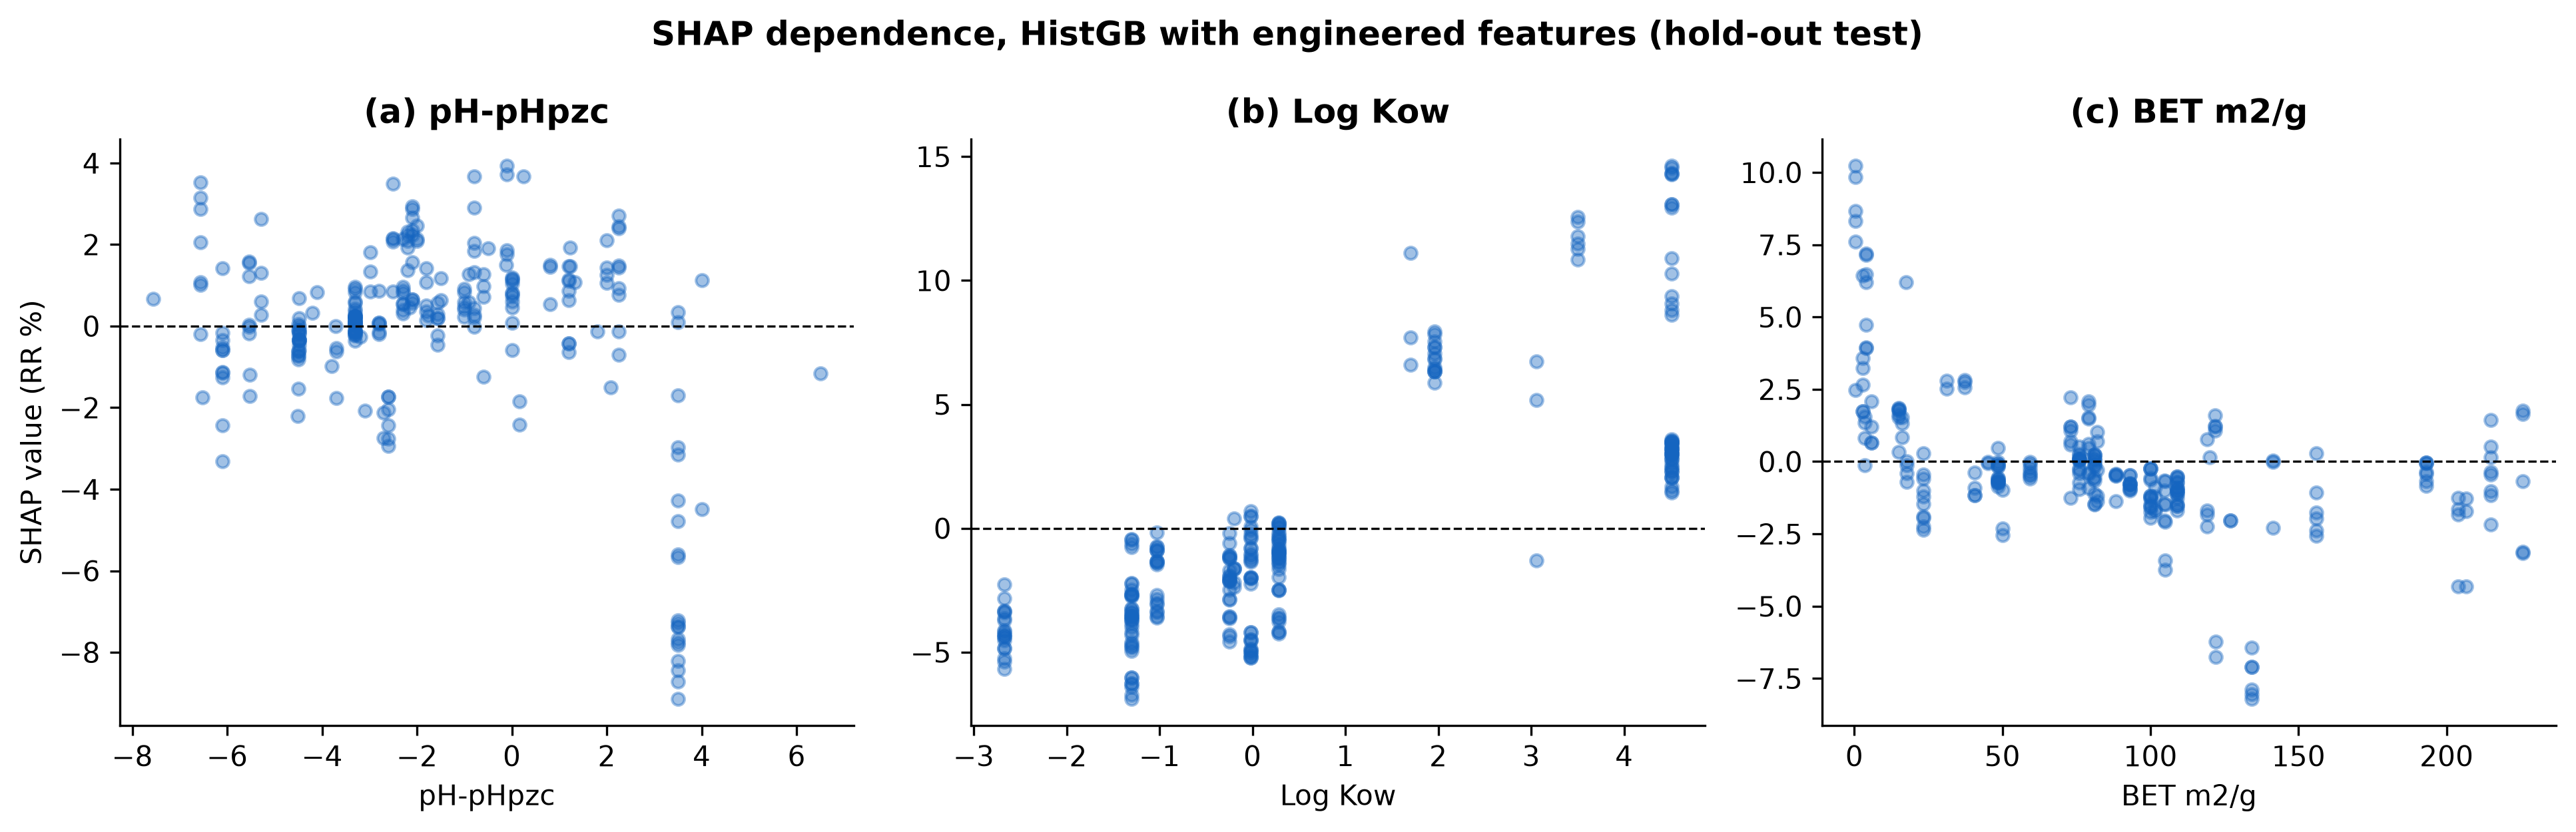
\includegraphics[width=\linewidth]{fig_shap_mechanism}
\caption{SHAP dependence of mechanism-linked features}
\label{fig:shap}
\end{figure}

\subsection{Computation time}
\label{sec:timing}

Training cost is not a differentiator at this data scale. On the
reference split, a single fit takes below one second for every model
except XGBoost (7--10~s across repeated measurements with the tuned
495-tree configuration), and prediction takes below 0.1~s throughout
(Table~S3). The full
leave-one-study-out audit, 59 refits of all seven models, completes
within minutes on a workstation, so the honest grouped protocol carries
no meaningful computational premium over the random-split protocol it
replaces. Hyperparameter search with Optuna dominates the overall
budget and is performed once, not per evaluation task.

\subsection{Environmental implications and outlook}
\label{sec:implications}

For practice, the results delimit two use cases sharply. Water-treatment
engineers optimizing operating conditions for an LDH--pollutant system
that has been measured before can rely on literature-trained models with
a mean absolute error near 6 percentage points of RR\%, tightened
further by conformal intervals. Materials researchers seeking to screen
new LDH formulations or new pollutants face a harder trade: the models
do carry transferable signal, reducing naive baseline errors by roughly
40 percent, but per-study skill remains near zero, so predictions for
unmeasured systems support coarse prioritization at best and should be
treated as hypotheses for experiment rather than estimates. Reported $R^2$ values
above 0.9 in prior compilations \citep{TODO-ml-adsorption-1,
TODO-biochar-cubist} are consistent with our record-level numbers and,
by the mechanism quantified here, likely overstate screening ability in
the same way; re-evaluation of published models under grouped protocols
would clarify how general this pattern is.

We see three concerns that temper the conclusions. First, the
compilation covers 59 studies, so the cross-study estimates themselves
carry sampling uncertainty; the per-study distribution, not a single
mean, is the honest summary. The second concern is reporting
heterogeneity between laboratories (differing protocols for
pH$_{\mathrm{pzc}}$ or BET), which acts as irreducible noise under (T2)
and may partly explain the transfer gap. The third concern is that our
descriptors, like those of prior compilations, describe the bulk
material; interlayer anion identity and surface morphology are rarely
reported and may carry the transferable signal that current models lack.
In future work, richer composition-structure descriptors, study-level
random effects, and few-shot calibration on a handful of measurements of
a new system are the most promising routes toward genuine screening
capability.

\section{Conclusions}
\label{sec:conclusions}

We evaluated seven machine learning models for micropollutant adsorption
on layered double hydroxides under a leakage-aware protocol that
separates within-system interpolation from cross-study generalization,
using 1,342 experiments compiled from 59 studies. The models predict
removal ratio for studied systems at new operating conditions with test
$R^2$ of $0.85 \pm 0.03$ and RMSE near 11 percentage points across 20
repeated splits, but the same models show near-zero per-study skill when
entire studies are held out, and a leave-one-study-out audit locates the
failure in a wide per-study error distribution rather than a uniform
degradation. Against descriptor-free baselines the picture is more
nuanced: the models reduce the naive cross-study error by roughly 40
percent, so they do carry transferable signal, yet not enough to certify
predictions for an unmeasured system. Split-conformal
intervals certify interpolation predictions at $\pm$19 percentage points,
whereas for unseen studies neither conformal calibration nor a
distance-based applicability score yields informative guarantees.
Chemistry-informed features such as pH$-$pH$_{\mathrm{pzc}}$ leave the
accuracy essentially unchanged but anchor the learned behavior in
electrostatic and hydrophobic mechanisms. In
future work, we plan to extend the compilation with interlayer-anion and
morphology descriptors, model study-level effects explicitly, and test
few-shot calibration so that a small number of measurements of a new
system can recover the accuracy currently reserved for studied ones.


\section*{CRediT authorship contribution statement}
[TO BE COMPLETED BY THE AUTHORS.]

\section*{Declaration of competing interest}
The authors declare that they have no known competing financial interests
or personal relationships that could have appeared to influence the work
reported in this paper.

\section*{Data availability}
The curated dataset, the full modeling pipeline
(\texttt{ldh\_pipeline.py}), and the notebooks reproducing every table and
figure are available at [REPOSITORY URL TO BE ADDED].

\bibliographystyle{elsarticle-harv}
\bibliography{main}

\end{document}
